\chapter{Binárne súbory a kompresia}
\label{sect:kompresia}

Doteraz sme na vstup a výstup používali objekty \vb{cin} a \vb{cout}, ktoré
sú tzv. {\em streamy}. Predstavujú štandardný vstup a výstup, za obvyklých
okolností sú to klávesnica a konzola, ale pri spúšťaní z príkazového riadka sa dajú 
presmerovať. Niekedy ale chceme priamo z programu písať do súboru. Na to existuje\indexItem{Prg}{\vb{fstream}}
knižnica \prg!fstream! (\prg!#include <fstream>!), v ktorej sú (okrem iného) definované
triedy \prg!ifstream! a \prg!ofstream! na čítanie a zapisovanie z/do súborov. S podobnou triedou \vb{stringstream} sme sa stretli
na str.~\pageref{here.stringstream}.
Tiredy \vb{ifstream} a \vb{ofstream} sa používajú
podobne. 

\begin{lstlisting}
#include <fstream>
#include <iostream>
using namespace std;

int main() {
  ifstream s("pako.txt");
  int x = -1;
  s >> x;
  cout << s.good() << " " << s.eof() << " " 
       << s.fail() << x << endl;
}
\end{lstlisting}


V tomto programe som vyrobil premennú \prg!s! typu \prg!istream! zviazanú so súborom
\vb{pako.txt} v aktuálnom adresári (t.j. tam, kde sa spúšťa binárka). 
Potom z neho skúšam načítať číslo. Trieda \prg!istream! má metódu \prg!bool good()!, ktorá
vždy povie, či je stream pripravený a metódu \prg!bool eof()!, ktorá hovorí, či bol
dosiahnutý koniec súboru. 
Ďalšia užitočná funkcia je \prg!fail()!, ktorá hovorí, či pri poslednom načítavaní
nastala chyba 
Vyskúšaj si spustiť tento program za rôznych okolností:
ak  súbor \vb{pako.txt} neexistuje, ak existuje, ale na začiatku nemá číslo, ale písmeno, 
ak existuje,
na začiatku má číslo a za ním nejaké znaky (napr. koniec riadka) a napokon ak existuje
a je v ňom iba jedno číslo (bez konca riadka). Všimni si, že ak raz nastane chyba a stream
prestane byť \vb{good}, už taký ostane, a \vb{eof} sa dosiahne, až keď sa pokúsi načítavať
za posledný znak v súbore. Ak chceš skončiť prácu so streamom, môžeš zavolať \prg!s.close()!.
Ak to nespravíš, všetko potrebné sa spraví v deštruktore (v našom prípade na konci programu).
Nasledovný program postupne prečíta zo súboru všetky čísla a vypíše ich:

\vskip 2ex
\vbox{
\begin{lstlisting}
#include <fstream>
#include <iostream>
using namespace std;

int main() {
  ifstream s("pako.txt");
  int x = -1;
  while (true) {
    s >> x;
    if (s.fail()) break;
    cout << x << endl;
  }
}
\end{lstlisting}
}

To isté sa dá docieliť aj jednoduchšie:

\begin{lstlisting}
  ifstream s("pako.txt");
  int x = -1;
  while (s >> x)
    cout << x << endl;
\end{lstlisting}

Čo znamená to \prg!while (s >> x)!? Podobne, ako sme v kapitole~\ref{sect:cukor}
pre náš typ \vb{Tabulka} definovali 

\begin{lstlisting}
ostream& operator <<(ostream& str , const Tabulka& o)
\end{lstlisting}

tak aj \prg!ifstream::operator>>(...)! vracia referenciu \prg!ifstream&!. Zároveň
má \prg!ifstream! definovaný 
\begin{lstlisting}
operator bool() {return !fail();}
\end{lstlisting}
ktorým sa dá hodnota\indexItem{Prg}{konverzia \vb{stream} na \vb{bool}}
\prg!ifstream! pretypovať na \prg!bool! (a výsledok je \prg!true! práve vtedy,
ak volanie \prg!fail! vráti \prg!false!). Takže zápis \prg!while (s >> x)! hovorí
\cmd{Prečítaj z \vb{s} celé číslo, ulož ho do \vb{x} a vráť referenciu na \vb{s}. 
Príkaz \vb{while} očakáva výraz typu \vb{bool}, 
preto zavolaj pretypovací operátor z \vb{ifstream}
a použi výslednú hodnotu.} Cyklus sa teda vykonáva, kým bolo načítanie úspešné.


Pretože \prg!ifstream! pracuje so súborom, nemusí, na rozdiel od \prg!cin! čítať súvisle\indexItem{Prg}{\vb{seekg}, \vb{tellg} a podobné}
za sebou. Dá sa predstaviť tak, že po súbore sa pohybuje kurzor, ktorý určuje miesto, z ktorého
sa práve ide čítať. Pozíciu kurzora vracia funkcia \prg!tellg()!. Kurzor sa dá posúvať
pomocou \prg!seekg()!, ktorá má dva parametre: prvý určuje o koľko sa má kurzor posunúť
a druhý odkiaľ sa má počítať: \prg!ios::beg! od začiatku súbora, \prg!ios::end! od konca, 
\prg!ios:cur! od súčasnej pozície. 
To \prg!ios::beg!, \prg!ios::end!, \prg!ios::cur! sú nejaké
konštanty, ktoré sú definované
v rámci \vb{namespace std::ios}; nebudeme teraz rozoberať, čo to presne je.
Vyskúšaj si napísať súbor \vb{pako.txt} s číslami,
medzerami a prázdnymi riadkami a spustiť si tento program:

\begin{lstlisting}
#include <fstream>
#include <iostream>
using namespace std;

int main() {
  ifstream s("pako.txt");
  int x = -1;
  s.seekg(0, ios::end);
  cout << "subor ma " << s.tellg() << " bytov." << endl;
  s.seekg(0, ios::beg);
  while (s >> x)
    cout << x << " a kurzor je na " << s.tellg() << endl;
}
\end{lstlisting}


Trieda \prg!ofstream! funguje podobne, 
s tým rozdielom, že vždy vytvorí nový súbor (ak súbor s daným
menom existoval, tak ho prepíše) a bude doňho zapisovať. Kvôli efektivite sa nezapisuje ihneď,
ale najprv do vyhradeného poľa v pamäti, ktoré sa do súboru zapíše až pri volaní \prg!close!.
Dá sa to ale urobiť aj skôr, zavolaním \prg!flush()!. Ak nechceš, aby sa súbor premazal,
môžeš použiť druhý parameter v konštruktore (resp. v \prg!open!), ktorým môžeš nastaviť
rôzne vlastnosti. Ak zavoláš \prg!ofstream s("pako.txt",ios:app);!, bude sa zapisovať na
koniec existujúceho súboru ({\em append}). Presúvať kurzor sa dá rovnako, ale namiesto
\prg!seekg! a \prg!tellg! treba\footnote{v skutočnosti netreba. Pre súborové streamy je vždy {\em put-pointer}
a {\em get-pointer} to isté, takže \vb{seekg} a \vb{seekp} urobí to isté. Ale napr. pre \vb{stringstream} to už neplatí,
takže je dobrý zvyk put- a get-pointer rozlišovať.
} použiť metódy \prg!seekp! a \prg!tellp!.


Súbory sa, rovnako ako pamäť, dajú predstaviť ako pole núl a jednotiek. Ak máš premennú
\prg!int x = 42!, v pamäti sú bity nastavené podľa dvojkového zápisu:
\vb{00101010} (a ešte ďalších 7 bytov samých núl, lebo \prg!int! má 8 bytov).
Operátory \prg!>>! a \prg!<<! ale čítajú a píšu textovú reprezentáciu: ak 
máš \prg!ofstream s;!
a napíšeš \prg!s << x!, do súboru sa napíšu dva byty: \vb{00110100} (čiže $52$) a 
\vb{00110010} (čiže $50$), čo sú ASCII kódy pre
znak \prg!'4'! a znak \prg!'2'!. Typy \prg!ifstream! a \prg!ofstream! umožňujú zapisovať \indexItem{Prg}{\vb{read} a \vb{write}}
a čítať aj priamo byty\footnote{%
  Ak pracuješ na inom systéme ako na Linuxe, operačný systém môže niektoré znaky (napr. 
  koniec riadku) prekladať inak. To znamená, že sa do súboru zapíše viac/iných znakov.
  Ak tento preklad nechceš, treba pri otváraní súboru použiť prepínač \prg!ios::binary!,
  napr. \prg!ifstream is("pako.txt", ios::in | ios::binary);! alebo
  \prg!ofstream os("pako.txt", ios::out | ios::binary);!. Všimni si, že na použitie
  viacerých prepínačov používam bitové OR. To je častá finta, ako v jednej premennej typu
  \prg!int! zapamätať niekoľko prepínačov: ak ich hodnoty sú mocniny dvojky, napr.
  \prg!int a=1, b=2, c=4, d=8;! tak každý z nich má v dvojkovom zápise iba jednu jednotku. 
  Preto napr. \prg!int x = b|d! je v dvojkovej sústave \vb{0010 | 1000}, čiže
  \vb{1010}, t.j. $10$.  Preto pre \prg!x=10! sú zapnuté prepínače \vb{b} a \vb{d}. 
  Otestovať, či je niektorý bit nastavený sa dá napr.
  \prg~if (x&d != 0) ...~.
  } pomocou funkcií \prg!read! a \prg!write!. Tie dostávajú ako parameter pointer na 
  \prg!char! a číslo $n$ a prečítajú resp. zapíšu $n$ bytov do/z pamäte. Samozrejme, 
  treba si dávať pozor, aby tá pamäť bola vhodne alokovaná, inak sa môže prepísať
  nejaká iná premenná (prípadne program spadne na segfault). 

   Vyskúšaj spustiť nasledovný program:
  
\begin{lstlisting}
#include <fstream>
#include <iostream>
using namespace std;

void zapis(long int x) {          
  ofstream s("pako.txt", ios::out | ios::binary);
  s.write((char *)&x, sizeof(x));
  s.close();                     // netreba, urobil by deštruktor
}

void citaj(long int &x) {        // toto \& znamená referenciu
  ifstream s("pako.txt", ios::in | ios::binary);
  s.read((char *)&x, sizeof(x)); // ale toto \& znamená adresu
  s.close();                     // netreba, urobil by deštruktor
}

int main() {
  long int x = 7020664791986103674;
  zapis(x);
  long int y;
  citaj(y);
  cout << y << endl;
  cout << sizeof(y) << endl;
}
\end{lstlisting}  

Teraz sa v nejakom editore pozri, čo sa vytvorilo v súbore \prg!pako.txt!.


Najmenšia jednotka, ktorá sa dá zapisovať a čítať je jeden byte, t.j. 8 bitov.
Aj typ \prg!bool!, ktorému by inak stačil 1 bit, má v pamäti (a v súbore)
veľkosť 1 byte. Nasledovný 
kus programu

\vskip 2ex
\vbox{
\begin{lstlisting}
bool a[40];
for (int i = 0; i < 20; i++) {
  a[2 * i] = false;
  a[2 * i + 1] = true;
}
ofstream s("pako.txt", ios::out | ios::binary);
s.write((char *)a, sizeof(a));
s.close();
\end{lstlisting}
}

preto do súboru \vb{pako.txt} zapíše 40 bytov s hodnotami striedavo 0 a 1.
Ak chceme zapisovať do súboru priamo bity, musíme to spraviť ``ručne''. Vyrobíme
si triedu \vb{BitWriter}, ktorá bude mať otvorený súbor na zápis a zároveň si bude
pamätať buffer \prg!buff!
na zapisovanie bitov: to môže byť napr. 8-bitový \prg!unsigned char! 
alebo 32-bitový \prg!unsigned int! alebo niečo iné, čo budeme mať ako šablónu
\prg!Buffer!.
Zároveň si budeme pamätať pozíciu bitu, ktorý práve nastavujeme ako \prg!int sz!,
takže ak máme pridať bit \prg!v! na koniec, zvýšime \prg!sz! a
spravíme \prg!(buff<<1)|(int)v!, čiže
posunieme binárny zápis \prg!buff! o 1 pozíciu doľava a na posledné miesto zapíšeme 
pomocou OR hodnotu \prg!v!. Ak zaplníme všetky bity, tak buffer zapíšeme do súboru
a vynulujeme. Ostáva jeden problém: na konci treba do súboru zapísať zostávajúci buffer,
ktorý doplníme nulami. Potom ale nevieme rozlíšiť, koľko núl bolo doplnených.
Môžme to spraviť tak, že na začiatok súboru napíšeme napr. \prg!long int len!, kde
si budeme pamätať celkovú dĺžku. Ako ju napísať na začiatok? Najprv tam zapíšeme 0,
aby sme mali v súbore urobené miesto a pred zatvorením súboru nastavíme kurzor
pomocou \prg!seekp! na začiatok a zapíšeme. Na zapisovanie bitu môžeme definovať
\prg!operator<<! a môžeme prihodiť aj verziu \prg!<<! pre čísla, ktorá postupne
zapíše všetky bity. Výsledok môže vyzerať nejak takto:

\begin{lstlisting}
template <typename Buffer = unsigned int>
struct BitWriter {
  ofstream f;
  Buffer buff;
  int sz;
  long int len;
  const int N = sizeof(Buffer);

  BitWriter(const string &fname) {
    f.open(fname, ios::out | ios::binary);
    sz = 0;
    buff = (Buffer)0;
    len = 0;
    f.write((char *)&len, sizeof(len));
  }

  ~BitWriter() {
    if (sz > 0) {    // zapíš do súboru zostávajúci buffer
      buff <<= 8 * N - sz;
      f.write((char *)(&buff), N);
    }
    f.seekp(0);     // na začiatok zapíšeme výslednú veľkosť
    f.write((char *)&len, sizeof(len)); 
    f.close();
  }

  BitWriter &operator<<(bool v) {
    buff = (buff << 1) | ((int)v);
    sz++;
    len++;
    if (sz == 8 * N) {
      f.write((char *)(&buff), N);
      sz = 0;
      buff = (Buffer)0;
    }
    return *this;
  }

  template <typename T>
  BitWriter &operator<<(const T &v) {
    for (int i = 8 * sizeof(T) - 1; i >= 0; i--)
      (*this) << ((v & (1 << i)) != 0);
    return *this;
  }
};
\end{lstlisting}

\begin{uloha}
  Naprogramuj analogickú triedu \vb{BitReader}, ktorá bude čítať (pomocou
  operátora \vb{>>}) to, čo \vb{BitWriter} zapísal. Pridaj \prg!operator bool(){...}!
  ktorý vráti \vb{true}, ak sa ešte nedočítalo do konca.
\end{uloha}

Nejaká verzia tried \vb{BitWriter} a \vb{BitReader} je v súbore
\link{\rootpath/bitwriter.h}{bitwriter.h}

\section*{Projekt: pakovač}
\label{projekt.pakovac}

Asi poznáš rôzne programy\footnote{napr. \vb{zip}, \vb{rar}, \vb{pkzip}, \vb{bzip2},
\vb{gzip}, \vb{7-zip} a mnohé iné}, ktoré zoberú veľký súbor a urobia z neho 
menší\footnote{väčšina z nich robí ešte veľa ďalších vecí, napr. že zabalí celý adresár
do jedného súboru, ale to nás teraz nebude zaujímať}. Ako to môže fungovať? Finta je v tom,
že nemôže. Povedzme, že chceme vedieť každý súbor s dĺžkou aspoň $1$ MiB (t.j. 
$1024\times1024=1048576$ bytov) skrátiť o $10$ bytov, t.j. vyrobiť kratší súbor, z ktorého
vieme ten pôvodný zrekonštruovať. Je jasné, že ak z dvoch rôznych pôvodných súborov $A$, $B$
dostaneme rovnaký skrátený súbor $X$, už je to celé v keli, lebo nevieme, či z $X$ sa má
zrekonštruovať $A$ alebo $B$. Čiže pre rôzne pôvodné súbory potrebujeme mať rôzne skrátené
súbory. Lenže všetkých súborov s dĺžkou $N$ bytov je $256^N$ (lebo jeden byte má $2^8=256$ 
rôznych hodnôt) a o $10$ bytov kratších súborov je iba $256^{N-10}$. Teda iba malý
zlomok $\frac{256^{N-10}}{256^N}=\frac{1}{256^{10}}\approx0.00000000000000000000008271\%$ 
všetkých
súborov vieme skrátiť. Zostávajúcu drvivú väčšinu 
\hbox{$\approx99.99999999999999999999991729\%$}
súborov neskrátime ani len o $10$ bytov, nech by sme robili čokoľvek.
Tak prečo tie programy fungujú? Súbory, ktoré používame, nie sú náhodné; väčšinu možných
súborov nikto nikdy nevytvorí, takže je nám srdečne jedno, že sa nedajú skrátiť. Nám záleží
na tom,
aby sa dalo skrátiť tých zopár málo, ktoré používame. 
Zober si napr. súbor 
\linkk{\rootpath/huff/demacek.txt}{\hbox{demacek.txt}}{Ondrej Demáček bol legendárny učiteľ 
informatiky, ktorý vychoval niekoľko generácií slovenských programátorov.}: 
má $81571$ bytov, ale používa 
iba $11$ rôznych znakov:  \prg!'.'!, \prg!':'!, \prg!'-'!, \prg!'='!, \prg!'+'!,
\prg!'*'!, \prg!'#'!, \prg!'%'!, \prg!'@'!
a k tomu medzera a koniec riadku. 
Pomocou jedného bitu vieme rozlíšiť dva znaky. Pomocou dvoch bitov štyri (lebo sú 4 kombinácie nuly a jednotky). Pomocou $k$
bitov vieme rozlíšiť $2^k$ znakov. Preto na uloženie textu, ktorý používa  $n$ rôznych znakov  by nám malo stačiť použiť $\log n$ bitov na zakódovanie jedného znaku.
Náš súbor ale na uloženie jedného znaku používa byte, t.j. 8 bitov,
aj keby stačilo $\log(11)\approx 3.45$ bitu\footnote{%
  Bit je predsa nula alebo jednotka, tak ako môžeme použiť $3.45$ bitu? Myslíme
  tým priemernú dĺžku na jeden znak. Ak by sme chceli zakódovať každý z 11 znakov, 
  potrebovali by sme $4$ bity na znak ($3$ nestačia, lebo nimi rozlíšime iba $2^3=8$ znakov). Ak by sme si ale povedali, že budeme
  kódovať dvojznakové kombinácie, ktorých je $11.11=121$, na jeden dvojznak by nám
  stačilo $7$ bitov ($2^7=128$), teda v priemere $\frac{7}{2}=3.5$ bitu na znak.
 Čím dlhšiu kombináciu
  znakov budeme kódovať naraz, tým viac sa budeme blížiť k hodnote $3.45$ na znak.
  }.
Keby sme si na začiatok súboru zaznačili znaky, ktoré používame, a potom používali iba 
ich čísla, súbor by sme skrátili na menej ako polovicu. Väčšina súborov, ktoré nás zaujímajú,
ale používa veľa rôznych znakov, takže touto fintou veľa neušetríme. Ale pravda je, že 
v súboroch spravidla nie sú všetky znaky zastúpené rovnomerne. Napr. v slovenskom
texte (s diakritikou)
\linkk{\rootpath/huff/dobsinsky.txt}{\hbox{dobsinsky.txt}}{tri diely Dobšinského rozprávok
zo servera \url{https://zlatyfond.sme.sk/}} tvorí $18$ najfrekventovanejších 
znakov\footnote{
  medzera, a, o, e, i, l, t, n, s, r, k, v, d, m, u, p, čiarka, h }
dokopy viac ako $80\%$ textu. V anglickom texte 
\linkk{\rootpath/huff/robinson.txt}{\hbox{robinson.txt}}{román Robinson Crusoe zo servera
\hbox{\url{https://www.gutenberg.org}}} je to ešte výraznejšie, $18$ najfrekventovanejších
znakov\footnote{medzera, e, t, o, a, n, h, i, s, r, d, l, u, m, w, čiarka,  c, f}
zaberá až viac ako $88\%$ textu. 
Aj v rámci frekventovaných znakov sú veľké rozdiely, nasledukúce grafy
ukazujú rozloženie početnosti najfrekventovanejších znakov:


\def\freqplot#1#2{
\begin{tikzpicture}
\begin{axis}[
    ybar interval,
    grid=none,
    ymajorgrids,
  width=\textwidth, 
  %ylabel=frekvencia \%,
  xlabel=\vb{#2},
    xtick={},
    xticklabels={,,},
    x tick label style={major tick length=0pt},
    y tick label style={},
    yticklabel={\pgfmathparse{\tick}\pgfmathprintnumber{\pgfmathresult}\%},
    xmin=0,
    ymin=0,
    xmax=50
]
  \addplot+[draw=blue!40!black,fill={rgb:blue,5;green,3;white,4}] 
  table [y=f, x=n]{data/#1_cnt.dat};
\end{axis}
\end{tikzpicture}
}

\begin{column}{0.45}
\freqplot{dobsinsky}{dobsinsky.txt}
\end{column}
\begin{column}{0.45}
\freqplot{robinson}{robinson.txt}
\end{column}

Programy sa správajú podobne ako prirodzený jazyk, vľavo je frekvencia početnosti znakov
pre súbor 
\link{\rootpath/huff/blender.src}{blender.src}, čo je 
zdrojový kód (v jazyku C++) grafického programu \link{https://www.blender.org/}{blender}.
Pre skompilované binárky je situácia horšia (graf vpravo je súbor 
\link{\rootpath/huff/wesnoth.bin}{wesnoth.bin}, čo je 
hlavná binárka hry \link{https://www.wesnoth.org/}{The Battle for Wesnoth}),
ale aj tam sa niektoré byty vyskytujú častejšie ako iné.


\begin{column}{0.45}
\freqplot{blender}{blender.src}
\end{column}
\begin{column}{0.45}
\freqplot{wesnoth}{wesnoth.bin}
\end{column}

\def\code#1{\textcolor{magenta}{\vb{#1}}}

 Ako vieme jednoducho využiť nerovnomernosti v zastúpení jednotlivých bytov\footnote{%
  V slovenskom texte je vzťah bytov a znakov trochu zložitejší, lebo používa kódovanie UTF8, v ktorom jeden 
  znak (napr. keď má diakritiku) môže zaberať viac bytov; navyše, ten istý znak ({\em glyf})
  sa dá niekedy zapísať rôznymi bytami. Nič z tohto nebudeme brať do úvahy a budeme pracovať 
  s bytami.}? Namiesto toho, aby sme každý znak zakódovali 8-bitovým číslom, môžeme znakom
  priradiť kódy (postupnosti núl a jednotiek) rôznej dĺžky. Znakom,
  ktoré sa vyskytujú častejšie, chceme priradiť kratšie kódy. Treba si ale dávať pozor, 
  aby sme to, čo zakódujeme, vedeli aj dekódovať. Napr. keby sme priradili kódy
  $a\mapsto\code{01}$ a $b\mapsto\code{0101}$, tak nevieme, či \code{0101} má byť
  $aa$ alebo $b$. Navyše chceme, aby sme zakódovaný súbor vedeli dekódovať efektívne.
Povedzme, že máme kód $a\mapsto\code{00}$, $b\mapsto\code{001}$, $c\mapsto\code{01}$
a $d\mapsto\code{10}$.
Keď vidíme začiatok postupnosti $\code{0010101\cdots}$ tak ju nevieme dekódovať, kým sa 
nepozrieme na koniec, lebo $\code{00101\cdots01}$ sa dekóduje ako $bccc\cdots c$, ale
$\code{00101\cdots010}$ sa dekóduje ako $addd\cdots d$.
Dobrý spôsob, ako zaručiť, že zakódovanú postupnosť 
budeme vedieť efektívne dekódovať, je navrhnúť kódy tak,\indexItem{Alg}{bezprefixový kód}
aby žiadny nebol začiatkom ({\em prefixom}) iného (napr. v našom poslednom príklade
je kód $a$čka \code{00} prefixom kódu $b$čka \code{001}. Každý takýto {\em bezprefixový}
kód si vieme nakresliť do stromu: koreň stromu bude zodpovedať všetkým kódom,
jeho ľavý syn všetkým kódom začínajúcim nulou a pravý syn kódom začínajúcim jednotkou.
Napríklad tento strom:


\centerline{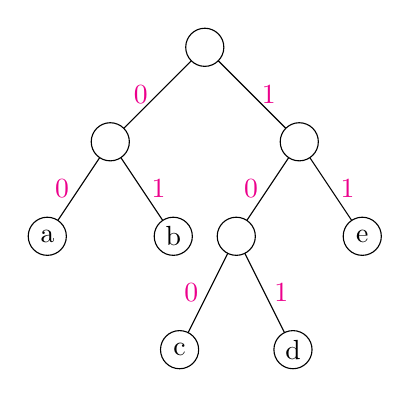
\begin{tikzpicture}[scale=0.8]
  \foreach \x/\y [count=\i] in {0/-1,
  -1.5/-2.5, 1.5/-2.5,
  -2.5/-4, -0.5/-4, 0.5/-4,2.5/-4,
  -0.4/-5.8, 1.4/-5.8
  } 
  \coordinate (n\i) at (\x,\y);

  \foreach \i/\j in {1/2,2/4,3/6, 6/8}
  \draw (n\i) -- node[anchor=east] {\textcolor{magenta}{\vb{0}}} (n\j);
  
  \foreach \i/\j in {1/3,2/5,3/7,6/9}
  \draw (n\i) -- node[anchor=west] {\textcolor{magenta}{\vb{1}}} (n\j);

  \foreach \i in {1,...,9}
  \filldraw[fill=white] (n\i) circle (2ex);

  \foreach \i/\a in {4/a,5/b,8/c,9/d,7/e}
  \node[draw=none] at (n\i) {\vb{\a}};
\end{tikzpicture}}


reprezentuje kód, ktorý priradí $a\mapsto\code{00}$, $b\mapsto\code{01}$,
$c\mapsto\code{100}$, $d\mapsto\code{101}$, $e\mapsto\code{11}$. Uvedom si, že ak
hodnoty jednotlivých znakov sú v listoch, tak kód je naozaj bezprefixový.
Naopak, každému stromu vieme priradiť bezprefixový kód. Takže kód a strom je v podstate to 
isté. Naša úloha je teraz takáto: máme daný text a chceme k nemu nájsť taký kód (t.j.
strom), že po zakódovaní dostaneme najkratší možný výstup. Ako to urobiť? Zoberme
si nasledovný text\footnote{Nie je to práve literárny skvost, ale chcel som, aby tam
bolo čo najmenej rôznych znakov.}:

\begin{verse}
\noindent
  \textcolor{rgb:blue,5;green,3;white,1}{\vb{%
ema ma mamu. mama ma malu emu ale ema nema lamu. mama ma lamu. mama a ema melu malu lamu. mala
lama nelame emu. emu lame eme lana. nela ema a lena melu lan. mama ma nulu. mama lame eme lamu.
  lama ma lunu. ela ma umelu lamu. lama ma mlela.%
  }}
\end{verse}

Jendotlivé znaky sa v texte vyskytujú takto:\\


\centerline{\begin{tabular}%
  {|>{\robotomono\textcolor{\stringcolor}\bgroup'}c<{'\egroup}|r|l@{\ \%\;}|}\hline
a&51&21.4286\\\hline 
\textvisiblespace&50&21.0084\\\hline
m&47&19.7479\\\hline
l&27&11.3445\\\hline
e&24&10.084\\\hline 
u&19&7.98319\\\hline
.&12&5.04202\\\hline 
n&8&3.36134\\\hline 
\end{tabular}}


\def\pis#1{\textcolor{\stringcolor}{\vb{'#1'}}}
Ako bude vyzerať dobrý strom? Určite písmeno \pis{n}, ktoré sa v texte vyskytuje najmenej,
dostane najdlhší kód. Prečo? Dajme tomu, že \pis{n} dostane kód dĺžky 3, ale \pis{l} dĺžky
5. Výskyty písmen \pis{n} a \pis{l} preto dokopy dajú $8\cdot3+27\cdot5=159$ bitov. 
Keby som ale všetky ostatné kódy nechal tak, a vymenil kódy \pis{n} a \pis{l}, písmená
 \pis{n} a \pis{l} budú dávať iba $8\cdot 5+27\cdot 3=121$ bitov.
Podobne druhý najdlhší kód bude mať druhý najzriedkavejší znak, \pis{.}. 
Dva najdlhšie kódy v strome majú znaky, ktoré sú v dvoch najspodnejších listoch. Teraz si 
všimni, že vždy sa dajú nájsť dva najhlbšie listy, ktoré majú spoločného rodiča. 
To znamená, že zatiaľ síce neviem, ako bude výsledný strom vyzerať, ale viem, že znaky
\pis{n} a \pis{.} budú na spodku stromu napr. takto (nezáleží na tom, ktorý
je vpravo a ktorý vľavo):\\


\centerline{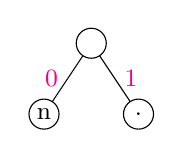
\begin{tikzpicture}[scale=0.6]
  \foreach \x/\y [count=\i] in {0/-1,
  -1/-2.5, 1/-2.5,
  } 
  \coordinate (n\i) at (\x,\y);

  \foreach \i/\j in {1/2}
  \draw (n\i) -- node[anchor=east] {\textcolor{magenta}{\small\roboto 0}} (n\j);
  
  \foreach \i/\j in {1/3}
  \draw (n\i) -- node[anchor=west] {\textcolor{magenta}{\small\roboto 1}} (n\j);

  \foreach \i in {1,...,3}
  \filldraw[fill=white] (n\i) circle (2.1ex);

  \foreach \i/\a in {2/n,3/.}
  \node[draw=none] at (n\i) {{\small\roboto \a}};
\end{tikzpicture}}


\def\psi{$\mathfrak{z}$}
\def\psii{$\mathfrak{y}$}
\def\psiii{$\mathfrak{d}$}
Ako bude vyzerať zvyšok stromu? Viem, že \pis{n} a \pis{.} majú rovnaký kód,
ktorý sa líši iba tým, že jeden má na konci nulu a druhý jednotku. Takže viem, že výsledný
text bude mať $8$-krát nulu (z kódov \pis{n}) a $12$-krát jednotku (z kódov \pis{.}).
Keď si odmyslím tieto posledné znaky, \pis{n} a \pis{.} sa správajú ako jedno
písmenko, napr. \pis{\psi}. Preto ak chcem nájsť najlepší strom pre celý text, stačí
mi nájsť najlepší strom pre nasledovný text:

\begin{verse}
\noindent
  \textcolor{rgb:blue,5;green,3;white,1}{\vb{%
ema ma mamu\psi{} mama ma malu emu ale ema \psi{}ema lamu\psi{} mama ma lamu\psi{} mama a ema melu malu lamu\psi{} mala lama \psi{}elame emu\psi{} emu lame eme la\psi{}a\psi{} \psi{}ela ema a le\psi{}a melu la\psi{}\psi{} mama ma \psi{}ulu\psi{} mama lame eme lamu\psi{} lama ma lu\psi{}u\psi{} ela ma umelu lamu\psi{} lama ma mlela\psi{}
  }}
\end{verse}

Spravím rovnakú úvahu: pozriem si početnosti jednotlivých znakov, zoberiem dva najmenej
početné (v tomto prípade \pis{\psi} a \pis{u}) a aktualizujem strom

\definecolor{donec}{rgb}{0.06, 0.3, 0.57}

\begin{column}{0.45}
\centerline{\begin{tabular}%
  {|>{\robotomono\textcolor{\stringcolor}\bgroup'}c<{'\egroup}|r|l@{\ \%\;}|}\hline
a&51&21.42866\\\hline
\textvisiblespace&50&21.0084\\\hline
m&47&19.74799\\\hline
l&27&11.34454\\\hline
e&24&10.084\\\hline
\psi&20&8.403368\\\hline
u&19&7.98319\\\hline
\end{tabular}}  
\end{column}
\hfill
\begin{column}{0.45}
\centerline{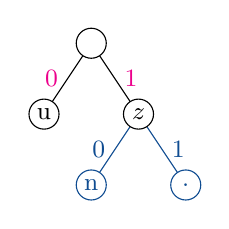
\begin{tikzpicture}[scale=0.6]
  \foreach \x/\y [count=\i] in {0/-1,
  -1/-2.5, 1/-2.5,
  -2/-1, -1/0.5
  } 
  \coordinate (n\i) at (\x,\y);

  % stare hrany
  \foreach \i/\j in {1/2}
  \draw[donec] (n\i) -- node[anchor=east] {\textcolor{donec}{\small\roboto 0}} (n\j);
  \foreach \i/\j in {1/3}
  \draw[donec] (n\i) -- node[anchor=west] {\textcolor{donec}{\small\roboto 1}} (n\j);
  
  % nove hrany
  \foreach \i/\j in {5/4}
  \draw (n\i) -- node[anchor=east] {\textcolor{magenta}{\small\roboto 0}} (n\j);
  \foreach \i/\j in {5/1}
  \draw (n\i) -- node[anchor=west] {\textcolor{magenta}{\small\roboto 1}} (n\j);

  % stare vrcholy
  \foreach \i in {2,3}
  \filldraw[draw=donec,fill=white] (n\i) circle (2.1ex);
  \foreach \i/\a in {2/n,3/.}
  \node[draw=none] at (n\i) {\textcolor{donec}{\small\roboto \a}};

  % nove vrcholy
  \foreach \i in {1,4,5}
  \filldraw[fill=white] (n\i) circle (2.1ex);
  \foreach \i/\a in {1/\psi,4/u,5/{}}
  \node[draw=none] at (n\i) {{\small\roboto \a}};
  
\end{tikzpicture}}
\end{column}


Opäť v texte spojím znaky \pis{\psi} a \pis{u} do nového znaku \pis{\psii} a dostanem text

\begin{verse}
\noindent
  \textcolor{rgb:blue,5;green,3;white,1}{\vb{%
ema ma mam\psii{}\psii{} mama ma mal\psii{} em\psii{} ale ema \psii{}ema lam\psii{}\psii{} mama ma lam\psii{}\psii{} mama a ema mel\psii{} mal\psii{} lam\psii{}\psii{} mala lama \psii{}elame em\psii{}\psii{} em\psii{} lame eme la\psii{}a\psii{} \psii{}ela ema a le\psii{}a mel\psii{} la\psii{}\psii{} mama ma \psii{}\psii{}l\psii{}\psii{} mama lame eme lam\psii{}\psii{} lama ma l\psii{}\psii{}\psii{}\psii{} ela ma \psii{}mel\psii{} lam\psii{}\psii{} lama ma mlela\psii{}
  }}
\end{verse}


Zistím si početnosti a zaradím dva najmenej početné znaky do stromu:


\begin{column}{0.45}
\centerline{\begin{tabular}%
  {|>{\robotomono\textcolor{\stringcolor}\bgroup'}c<{'\egroup}|r|l@{\ \%\;}|}\hline
a&51&21.42866\\\hline
\textvisiblespace&50&21.0084\\\hline
m&47&19.74799\\\hline
\psii&39&16.3866\\\hline
l&27&11.3445\\\hline
e&24&10.084\\\hline
\end{tabular}}
\end{column}
\hfill
\begin{column}{0.45}
\centerline{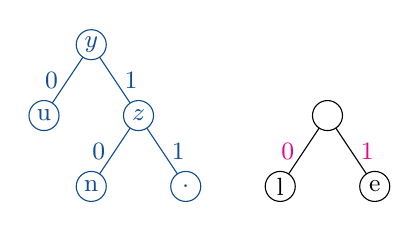
\begin{tikzpicture}[scale=0.6]
  \foreach \x/\y [count=\i] in {0/-1,
  -1/-2.5, 1/-2.5,
  -2/-1, -1/0.5,
  3/-2.5, 5/-2.5, 4/-1
  } 
  \coordinate (n\i) at (\x,\y);

  % stare hrany
  \foreach \i/\j in {1/2, 5/4}
  \draw[donec] (n\i) -- node[anchor=east] {\textcolor{donec}{\small\roboto 0}} (n\j);
  \foreach \i/\j in {1/3, 5/1}
  \draw[donec] (n\i) -- node[anchor=west] {\textcolor{donec}{\small\roboto 1}} (n\j);
  
  % nove hrany
  \foreach \i/\j in {8/6}
  \draw (n\i) -- node[anchor=east] {\textcolor{magenta}{\small\roboto 0}} (n\j);
  \foreach \i/\j in {8/7}
  \draw (n\i) -- node[anchor=west] {\textcolor{magenta}{\small\roboto 1}} (n\j);

  % stare vrcholy
  \foreach \i in {1,...,5}
  \filldraw[draw=donec,fill=white] (n\i) circle (2.1ex);
  \foreach \i/\a in {2/n,3/.,1/\psi,4/u,5/\psii}
  \node[draw=none] at (n\i) {\textcolor{donec}{\small\roboto \a}};

  % nove vrcholy
  \foreach \i in {6,...,8}
  \filldraw[fill=white] (n\i) circle (2.1ex);
  \foreach \i/\a in {6/l,7/e,8/{}}
  \node[draw=none] at (n\i) {{\small\roboto \a}};
  
\end{tikzpicture}}
\end{column}


Teraz som dostal dva nesúvislé kusy stromu, ale to mi nijak nevadí: viem, že vo výsledom 
strome bude kdesi visieť jeden kus a kdesi inde druhý. Pokračujem rovnako ďalej, spojím
\pis{l} a \pis{e} do jedného znaku \pis{\psiii}:

\begin{verse}
\noindent
  \textcolor{rgb:blue,5;green,3;white,1}{\vb{%
\psiii{}ma ma mam\psii{}\psii{} mama ma ma\psiii{}\psii{} \psiii{}m\psii{} a\psiii{}\psiii{} \psiii{}ma \psii{}\psiii{}ma \psiii{}am\psii{}\psii{} mama ma \psiii{}am\psii{}\psii{} mama a \psiii{}ma m\psiii{}\psiii{}\psii{} ma\psiii{}\psii{} \psiii{}am\psii{}\psii{} ma\psiii{}a \psiii{}ama \psii{}\psiii{}\psiii{}am\psiii{} \psiii{}m\psii{}\psii{} \psiii{}m\psii{} \psiii{}am\psiii{} \psiii{}m\psiii{} \psiii{}a\psii{}a\psii{} \psii{}\psiii{}\psiii{}a \psiii{}ma a \psiii{}\psiii{}\psii{}a m\psiii{}\psiii{}\psii{} \psiii{}a\psii{}\psii{} mama ma \psii{}\psii{}\psiii{}\psii{}\psii{} mama \psiii{}am\psiii{} \psiii{}m\psiii{} \psiii{}am\psii{}\psii{} \psiii{}ama ma \psiii{}\psii{}\psii{}\psii{}\psii{} \psiii{}\psiii{}a ma \psii{}m\psiii{}\psiii{}\psii{} \psiii{}am\psii{}\psii{} \psiii{}ama ma m\psiii{}\psiii{}\psiii{}a\psii{}
  }}
\end{verse}


\begin{column}{0.45}
\centerline{\begin{tabular}%
  {|>{\robotomono\textcolor{\stringcolor}\bgroup'}c<{'\egroup}|r|l@{\ \%\;}|}\hline
a&51&21.42866\\\hline
\psiii&51&21.4286\\\hline
\textvisiblespace&50&21.0084\\\hline
m&47&19.74799\\\hline
\psii&39&16.3866\\\hline
\end{tabular}}
\end{column}
\hfill
\begin{column}{0.45}
\centerline{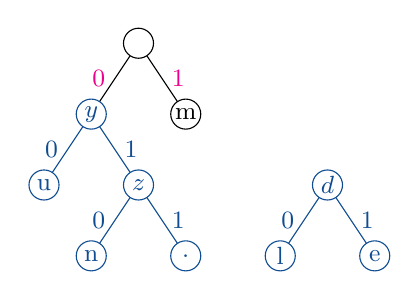
\begin{tikzpicture}[scale=0.6]
  \foreach \x/\y [count=\i] in {0/-1,
  -1/-2.5, 1/-2.5,
  -2/-1, -1/0.5,
  3/-2.5, 5/-2.5, 4/-1,
  1/0.5, 0/2
  } 
  \coordinate (n\i) at (\x,\y);

  % stare hrany
  \foreach \i/\j in {1/2, 5/4,8/6}
  \draw[donec] (n\i) -- node[anchor=east] {\textcolor{donec}{\small\roboto 0}} (n\j);
  \foreach \i/\j in {1/3, 5/1, 8/7}
  \draw[donec] (n\i) -- node[anchor=west] {\textcolor{donec}{\small\roboto 1}} (n\j);
  
  % nove hrany
  \foreach \i/\j in {10/5}
  \draw (n\i) -- node[anchor=east] {\textcolor{magenta}{\small\roboto 0}} (n\j);
  \foreach \i/\j in {10/9}
  \draw (n\i) -- node[anchor=west] {\textcolor{magenta}{\small\roboto 1}} (n\j);

  % stare vrcholy
  \foreach \i in {1,...,8}
  \filldraw[draw=donec,fill=white] (n\i) circle (2.1ex);
  \foreach \i/\a in {2/n,3/.,1/\psi,4/u,5/\psii,6/l,7/e,8/\psiii}
  \node[draw=none] at (n\i) {\textcolor{donec}{\small\roboto \a}};

  % nove vrcholy
  \foreach \i in {9,10}
  \filldraw[fill=white] (n\i) circle (2.1ex);
  \foreach \i/\a in {9/m,10/{}}
  \node[draw=none] at (n\i) {{\small\roboto \a}};
  
\end{tikzpicture}}
\end{column}


Takto budem postupne zdola nahor vytvárať strom: vždy spojím dve najmenej početné znaky do 
jedného a zlepím príslušné kusy stromu spoločným vrcholom, až dostanem napr. strom:


\def\stromzobrazka{%
\centerline{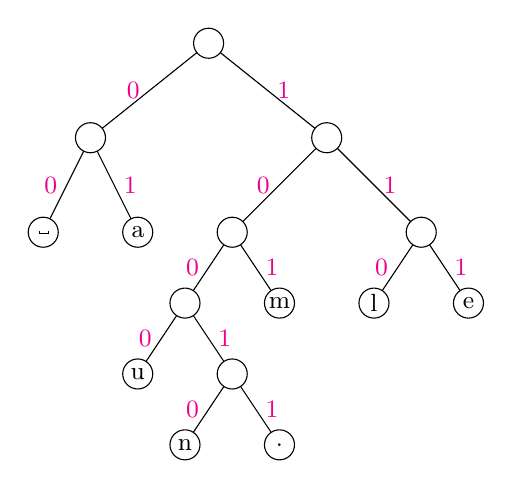
\begin{tikzpicture}[scale=0.6]
  \foreach \x/\y [count=\i] in {0/-1,
  -1/-2.5, 1/-2.5,
  -2/-1, -1/0.5,
  3/0.5, 5/0.5, 4/2,
  1/0.5, 0/2,
  2/4,
  -4/2, -2/2, -3/4, -0.5/6 
  } 
  \coordinate (n\i) at (\x,\y);

  \foreach \i/\j in {10/5,1/2, 5/4,8/6,11/10,14/12,15/14}
  \draw (n\i) -- node[anchor=east] {\textcolor{magenta}{\small\roboto 0}} (n\j);
  \foreach \i/\j in {10/9,1/3, 5/1, 8/7,11/8,14/13,15/11}
  \draw (n\i) -- node[anchor=west] {\textcolor{magenta}{\small\roboto 1}} (n\j);

  \foreach \i in {1,...,15}
  \filldraw[fill=white] (n\i) circle (2.1ex);
  \foreach \i/\a in {2/n,3/.,1/{},4/u,5/{},6/l,7/e,8/{},9/m,10/{},11/{},
  12/{\textvisiblespace},13/a,14/{},15/{}}
  \node[draw=none] at (n\i) {{\small\roboto \a}};
\end{tikzpicture}}}
\stromzobrazka


Táto metóda je známa pod menom {\em Huffmanovo} kódovanie. Poďme ju teraz skúsiť\indexItem{Alg}{Huffmanovo kódovanie}
naprogramovať. Najprv sa treba rozhodnúť, ako budeme v pamäti reprezentovať strom,
ktorý vytvárame. Spravme si takýto typ:

\begin{lstlisting}
struct Item {
  unsigned char val;
  int par = -1, freq = 0;
  int l = -1, r = -1;
};
\end{lstlisting}

v ktorom si o každom znaku budeme pamätať jeho hodnotu (\prg!char val!) a početnosť 
(\prg!int freq!). Tieto znaky budeme mať uložené v poli a hodnoty \prg!par, l, r! budú
indexy rodiča, ľavého a pravého syna. Takže strom z obrázka hore by mohol
vyzerať napr. takto:


\centerline{
\begin{tikzpicture}[xscale=0.9,yscale=0.5]
    \def\cmd(#1)#2{
      \begin{scope}[shift={(#1,0)}]
        \draw (0,-0.1) rectangle (1,5.2);
        \foreach \v [count = \i] in {#2}{
          \node [anchor=south] at (0.5,\i-1) {\vb{\textcolor{magenta}{\v}}};
        }
        \node [anchor=south] at (0.5,5.2) {$#1$};
      \end{scope}
      }

  \foreach \l [count = \i] in {r,l,par,freq,val}
   \node [anchor=south east] at (0,\i-1) {\vb{\l}};

  \cmd(0){-1,-1,10,27,\pis{l}}
  \cmd(1){-1,-1,8,12,\pis{.}}
  \cmd(2){-1,-1,9,19,\pis{u}}
  \cmd(3){-1,-1,8,8,\pis{n}}
  \cmd(4){-1,-1,12,50,\pis{\textvisiblespace}}
  \cmd(5){-1,-1,12,51,\pis{a}}
  \cmd(6){-1,-1,11,47,\pis{m}}
  \cmd(7){-1,-1,10,24,\pis{e}}
  \cmd(8){3,1,9,20,{}}
  \cmd(9){2,8,11,39,{}}
  \cmd(10){0,7,13,51,{}}
  \cmd(11){9,6,13,86,{}}
  \cmd(12){4,5,14,101,{}}
  \cmd(13){11,10,14,137,{}}
  \cmd(14){12,13,-1,238,{}}
\end{tikzpicture}
}


Ako takéto pole vyrobíme? Začiatok je ľahký: prečítame vstupný súbor do poľa znakov,
prejdeme cez neho a pre každý znak (je ich iba 256 možných) si v pomocnom poli \vb{freq}
budeme pamätať, koľkokrát sa tam príslušný znak vyskytuje. Nakoniec pre každý znak,
ktorý má nenulový počet výskytov pridáme jeden \vb{item}:

\begin{lstlisting}
ifstream f(src, ios::in | ios::binary);
f.seekg(0, ios::end);
vector<unsigned char> text(f.tellg());
f.seekg(0, ios::beg);
f.read((char *)(text.data()), text.size());

vector<int> freq(256, 0);
for (unsigned char c : text) freq[c]++;

vector<Item> items;
for (int i = 0; i < 256; i++) if (freq[i] > 0) 
    items.push_back({(unsigned char)i, -1, freq[i], -1, -1});
\end{lstlisting}


Ďalej budeme potrebovať opakovane spájať najmenej početné znaky. Budeme na to potrebovať\indexItem{Alg}{halda ({\em heap})}
dátovú štruktúru, kde vieme 1) vložiť znak a 2) odobrať znak s najmenšou početnosťou. 
Takáto dátová štruktúra sa volá {\em halda} ({\em heap}) a ľahko by sme si ju 
vedeli naprogramovať v poli, ale keď máme v ruke kladivo (typ \vb{set}), tak všetko
vyzerá ako klinec: spravíme si premennú \vb{heap}  typu \vb{set}. 
Treba si ale premyslieť, čo budeme do nej
ukladať. Na jednej strane potrebujeme, aby boli prvky usporiadané podľa početnosti. 
Na druhej strane, keď zoberieme najmenej početný znak (hodnotu \vb{*heap.begin()}),
potrebujeme na základe nej vedieť upraviť pole \vb{items}. Použijeme jednoduchú fintu,
ktorú umožňuje verzia typu \vb{set} s porovnávacou funkciou: v premennej \vb{heap}
si budeme ukladať iba indexy do poľa \vb{items} a porovnávacia funkcia 
sa bude rozhodovať podľa hodnoty \vb{items[i].freq}:

\begin{lstlisting}
multiset<int, function<bool(int, int)>> heap(
    [&items](int i, int j) { 
        return items[i].freq < items[j].freq; 
    });
\end{lstlisting}

Tento zápis hovorí, že používam šablónu na ukladanie typu \prg!int! s tým,
že v konštruktore pridám porovnávaciu funkciu typu \prg!function<bool(int, int)>!,
t.j. lambdu, ktorá zoberie dva parametre typu \prg!int! a vráti \prg!bool!.
Vzápätí takú premennú s menom \prg!heap! vyrobím, a v konštruktore 
jej pridám lambdu, ktorá má ako {\em capture} referenciu\footnote{%
  to je dôležité: zápis \vb{[items](\prg!int i,int j!)\{...\}} by do lambdy
zobral hodnotu \vb{items}, t.j. 
lokálnu kópiu poľa \vb{items}, ako vyzeralo v čase volania konštruktora}
  na pole \vb{items}:
\prg![&items](int i, int j) {...}!. Preto v tele lambdy viem pristupovať k poľu
\vb{items} a porovnávať dva prvky \vb{i} a \vb{j} podľa početností znakov
\prg!items[i].freq! a \prg!items[j].freq!. Tu si ale treba dať dobrý pozor a uvedomiť si
čo sa deje: v type \vb{set} sa pracuje s vyvažovaným stromom, kde v uzloch sú uložené
čísla. Vždy, keď treba dve čísla porovnať, tak namiesto \vb{<} sa zavolá príslušná
lambda. To znamená, že ak by sme zmenili hodnoty \vb{freq} v poli \vb{items}, strom, 
ktorý je vyrobený v \vb{heap} už nebude správny. Preto hodnoty v \vb{items} musíme 
meniť tak, že najprv odoberieme z \vb{heap} index, ktorého frekvenciu chceme zmeniť,
potom zmeníme frekvenciu, a potom index znovu pridáme do \vb{heap}, takže všetky porovnania,
ktoré sa v strome \vb{heap} robia, budú konzistentné. Ešte si treba uvedomiť, 
že v \vb{heap} síce budeme mať uložené rôzne čísla (indexy do \vb{items}), ale 
porovnávame ich podľa našej funkcie, a keďže môžeme mať viacero znakov s rovnakou
frekvenciou, potrebujeme použiť typ \vb{multiset}. Pri vytváraní poľa \vb{items}
si zároveň pripravíme pole \vb{idx}, ktoré použijeme neskôr pri samotnom vytváraní kódu:
pre každý znak \prg!c! mám v \prg!idx[c]! uložené, kde v \vb{items} je príslušný list.
Celý kus kódu môže vyzerať takto:

\begin{lstlisting}
vector<int> idx(256, -1);
for (int i = 0; i < 256; i++) if (freq[i] > 0) {
    int n = items.size();
    items.push_back({(unsigned char)i, -1, freq[i], -1, -1});
    heap.insert(n);
    idx[i] = n;
}
int n_chars = items.size(); // počet listov stromu

while (heap.size() > 1) {
  int i = pop(heap);
  int j = pop(heap);
  int n = items.size();
  items.push_back({0, -1, items[i].freq + items[j].freq});
  items[i].par = items[j].par = n;
  heap.insert(n);
}
\end{lstlisting}


Funkcia \vb{pop} je len jednoduchá pomocná funkcia, aby som ušetril písanie, napr. takto:

\begin{lstlisting}
template <typename T>
int pop(T &heap) {
  int u = *heap.begin();
  heap.erase(heap.begin());
  return u;
}
\end{lstlisting}


Zatiaľ máme v poli \vb{items} nastavených rodičov, ale ešte sme nenastavovali
položky \vb{l} a \vb{r}. Tie môžeme nastaviť napr. takto:

\begin{lstlisting}
for (int i = 0; i < items.size(); i++)
  if (items[i].par != -1) {
    if (items[items[i].par].l == -1)
      items[items[i].par].l = i;
    else
      items[items[i].par].r = i;
  }
\end{lstlisting}


Keď máme hotové pole \vb{items}, chceme pre každý znak vyrobiť jeho kód. To je
jednoduché: postupujeme smerom k rodičovi a podľa toho, či to bol ľavý alebo
pravý syn, priradíme 0 alebo 1. Nakoniec kód obrátime, lebo ho chceme mať smerom
od koreňa k listom:

\begin{lstlisting}
vector<vector<bool>> code(n_chars);

for (int i = 0; i < n_chars; i++)
  for (int j = i; items[j].par != -1; j = items[j].par)
    if (items[items[j].par].l == j)
      code[i].push_back(true);
    else
      code[i].push_back(false);

for (auto &x : code) reverse(x.begin(), x.end());
\end{lstlisting}


Do výstupného súboru potrebujeme zapísať kód každého znaku zo vstupu tak, ako idú za sebou. Potrebujeme ale
nejak zapísať aj ''slovník'', t.j. pre každý možný znak zapísať jeho kód. Ten chceme zapísať 
tak, aby sme použili čo najmenej bitov a pritom bolo jednoduché ho zapísať aj prečítať.
Dá sa to urobiť napr. tak, že zapíšeme rekurzívne celý strom: ak sme v liste, zapíšeme
bit \vb{1} a za ním znak (8 bitov). Ak sme vo vnútornom vrchole, zapíšeme bit \vb{0}
a za ním rekurzívny zápis ľavého a pravého podstromu. Strom z nášho príkladu:


\stromzobrazka


by sme zapísali \vb{0\textcolor{blue!60!white}{01\textvisiblespace1a}0001u01n1.1m01l1e}.
Pri dekódovaní najprv prečítame slovník do premennej typu \vb{*Node}

\begin{lstlisting}
struct Node {
  unsigned char val;
  Node *l, *r;
  Node() : l(nullptr), r(nullptr) {}
  ~Node() {
    if (l) delete l;
    if (r) delete r;
  }
};
\end{lstlisting}

Samotné dekódovanie je priamočiare: čítame bity, prechádzame stromom a vždy, keď prídeme
do listu, vypíšeme príslušný znak:

\begin{lstlisting}
void decompress(const string &src, const string &dst) {
  BitReader<> in(src);
  ofstream dstf(dst, ios::out | ios::binary);
  Node *root = readTree(in);
  for (Node *p = root; in;) {
    bool v;
    in >> v;
    if (v)
      p = p->l;
    else
      p = p->r;
    if (p->l == nullptr) {
      dstf.write((char *)&(p->val), 1);
      p = root;
    }
  }
}
\end{lstlisting}


Nakoniec by sme chceli vyrobiť program, ktorý vie kódovať a dekódovať podobne, ako 
štandardné programy, teda funguje z príkazového riadka ({\em CLI, command line interface}).
Zatiaľ vieme skompilovať program, ktorý keď sa spustí, číta zo štandardného vstupu
alebo zo súboru. Ale veľakrát vidíš programy, ktoré čítajú parametre
priamo pri spustení, napr. \vb{gzip -k subor.txt}
Tieto parametre operačný systém posiela programu ako parametre funkcie \vb{main}.\indexItem{Prg}{parametre z príkazového riadka}
Ak v programe namiesto \vb{int main() ...} napíšeš \hbox{\vb{int main (int argc, char** argv)...}}
premenná \vb{argc } bude obsahovať počet argumentov a premenné \vb{argv[0]},
\vb{argv[1]},\ldots,\vb{argv[argc-1]} postupne všetky parametre (ako reťazce znakov 
\prg!char *! alokované kdesi v systémovej pamäti) s tým, že \vb{argv[0]} je názov
binárky, t.j. pre príklad \vb{gzip -k subor.txt} je \prg!argc==3!, \prg!argv[0]=="gzip"!,
\prg!argv[1]=="-k"! a \prg!argv[2]=="subor.txt"!.

\begin{uloha}
  Naprogramuj Huffmanovu kompresiu. Program má dostať ako parametre zdrojový súbor a cieľový
  súbor. Ak je spustený s prepínačom \vb{-d} má dekódovať, inak kódovať.
\end{uloha}

Po naprogramovaní vyzerajú veľkosti súborov takto:\\


\def\line#1#2#3{\vb{#1}&$#2$&$#3$&$\calc[precision=3]{8*#3/#2}$&%
$\calc[precision=2]{100*#3/#2}\;\%$\\}
\centerline{
  \begin{tabular}{|l|r|r|r|r|}\hline
    súbor & pôvodne (B) & Huffman (B) & bit/znak& kompresia \\\hline
    \line{blender.src}{54259819}{35354132}
    \line{demacek.txt}{81571}{31013}
    \line{dobsinsky.txt}{2045382}{1266856}
    \line{robinson.txt}{659018}{369272}
    \line{wesnoth.bin}{22159352}{16074583}\hline
  \end{tabular}
}


Jednou z nevýhod tohto kódovania je, že neberie do úvahy závislosti medzi znakmi. 
Napr. v slovenčine je \pis{y} pomerne častý znak, ale po \pis{š} nejde takmer nikdy.
Preto \pis{y} by mohlo dostávať rôzne dlhý kód v závislosti od toho, čo bolo pred ním.
Mohli by sme to urobiť tak, že si vyrobíme veľa nezávislých Huffmanových kódov: pre každé
predchádzajúce písmenko (tzv. {\em kontext}) jeden a pri kódovaní a dekódovaní
vždy použijeme ten správny. Problém je, že ak by sme chceli mať kontext dlhší, napr.
2, 3, či viac predchádzajúcich písmen, počet Huffmanovských stromov (a teda aj slovníkov, ktoré musím mať zapísané v súbore) bude veľmi narastať. 
Iná možnosť, ako docieliť podobný efekt, je z takejto úvahy: ak by som mal program \indexItem{Alg}{kompresia s prediktorom}
({\em prediktor}), ktorý
vie vždy z doterajšieho textu povedať, aké písmenko bude nasledovať, tak netreba nič 
komprimovať, prediktor mi súbor rovno vygeneruje.
Nedúfam, že taký prediktor budem mať, ale čo ak by som 
mal nie celkom dokonalý, ale stále dosť dobrý prediktor? Taký, ktorý dosť často trafí, aké písmenko
bude nasledovať, a ak sa aj netrafí, nebude od skutočného písmenka moc ďaleko. Na zrekonštruovanie pôvodného
textu by som potom nepotreboval kódovať znaky zo vstupu, stačlo by mi pre každý vstupný znak zakódovať chybu, ktorú prediktor spravil. Na základe toho 
by som už vedel znak zo vstupu zrekonštruovať\footnote{%
 Pri kódovani sa vždy pozriem, aké písmenko predikuje prediktor a aké písmenko je v skutočnosti na vstupe. Chybu zakódujem na výstup a aktualizujem prediktor.
 Pri dekódovaní je to podobné: pozriem sa, čo hovorí prediktor, zo vstupu dekódujem chybu, z nej vyrobím skutočné písmenko, vypíšem ho na dekódovaný výstup a
 zároveň pomocou neho aktualizujem prediktor.
}. 
Ak je prediktor dobrý,
môžem dúfať, že chyby budú väčšinou nuly, a teda sa budú dať skomprimovať lepšie, ako 
pôvodný súbor. Ako spraviť prediktor? Môžem si napríklad pre každý kontext (niekoľko predchádzajpúcich písmeniek)
pamätať znaky usporiadané podľa početnosti, koľkokrát som ktorý v danom kontexte videl.
Prediktor potom vráti poradie znaku v tomto usporiadaní. Ak je napr. kontext \vb{nsk},
a pamätám si usporiadanie písmen \vb{ý, é, á, ú, o, a, ... } a na vstupe je ako
ďalšie písmenko \vb{o}, prediktor vráti $4$, lebo to je poradie \vb{o} v tomto kontexte.

\begin{uloha}
  Naprogramuj takýto prediktor.
\end{uloha}

Ak sa pozrieš, ako tento prediktor funguje pre kontext troch písmeniek, vidno, že po 
predspracovaní súborov sa frekvencie znakov výrazne zmenia (priesvitné modré stĺpce
sú pôvodné frekvencie bez prediktora, zelené s prediktorom)

\def\freqplot#1#2{
\begin{tikzpicture}
\begin{axis}[
    grid=none,
    ymajorgrids,
  width=\textwidth, 
  %ylabel=frekvencia \%,
  xlabel=\vb{#2},
    xtick={},
    xticklabels={,,},
    x tick label style={major tick length=0pt},
    y tick label style={},
    yticklabel={\pgfmathparse{\tick}\pgfmathprintnumber{\pgfmathresult}\%},
    xmin=0,
    ymin=0,
    ymax=65,
    xmax=20
]
  \addplot+[ybar interval,draw=green!40!black,fill={rgb:red,3;green,7;white,4},
  mark size=0] 
  table [y=f, x=n]{data/#1_prd_cnt.dat};
  \addplot+[ybar interval, draw=blue!40!black, fill={rgb:blue,5;green,3;white,9}, 
  opacity=0.6, mark size=0] 
  table [y=f, x=n]{data/#1_cnt.dat};
\end{axis}
\end{tikzpicture}
}


\begin{column}{0.45}
\freqplot{dobsinsky}{dobsinsky.txt}
\end{column}
\begin{column}{0.45}
\freqplot{robinson}{robinson.txt}
\end{column}

\begin{column}{0.45}
\freqplot{blender}{blender.src}
\end{column}
\begin{column}{0.45}
\freqplot{wesnoth}{wesnoth.bin}
\end{column}


Keď teraz Huffmanovým pakovačom skomprimujem výsledky prediktora, dostnem lepšiu kompresiu:\\

\def\tmp#1#2{$\calc[precision=3]{8*#2/#1}$&$\calc[precision=2]{100*#2/#1}\;\%$}
\def\line#1#2#3#4#5{\vb{#1}&\tmp{#2}{#3}&\tmp{#2}{#4}&\tmp{#2}{#5}\\}
\def\lbl{& bit/znak& kompresia }
\centerline{
  \begin{tabular}{|c|r|r|r|r|r|r|}\hline
    \multirow{2}{*}{súbor}
    &\multicolumn{2}{c|}{Huffman}&\multicolumn{2}{c|}{Huffman s prediktorom}&
    \multicolumn{2}{c|}{\vb{gzip}}\\\cline{2-7}
     \lbl\lbl\lbl \\\hline
    \line{blender.src}{54259819}{35354132}{16621515}{10570257}
    \line{demacek.txt}{81571}{31013}{13864}{12312}
    \line{dobsinsky.txt}{2045382}{1266856}{773429}{788664}
    \line{robinson.txt}{659018}{369272}{239737}{246535}
    \line{wesnoth.bin}{22159352}{16074583}{10270957}{7402770}\hline
  \end{tabular}
}


Ako vidíš, prediktor výrazne pomohol kompresii, v niektorých prípadoch je výsledok
lepší ako \vb{gzip}\footnote{aj keď beží o dosť pomalšie}. 
Väčšina kompresných algoritmov používa buď Huffmanovo kódovanie
kombinované s tzv. {\em run-length encoding}\footnote{%
  Huffmanov kód z princípu nevie urobiť menšiu ako 8-násobnú kompresiu, lebo na každý
  znak použije aspoň 1 bit. Ak je vo vstupnom súbore dlhá postupnosť rovnakých znakov,
  napr. \vb{0000000000000}, je lepšie ju nahradiť \vb{[13]0} s významom \cmd{trinásťkrát
  zopakuj nulu}.} alebo algoritmy, ktoré kódujú nie jednotlivé znaky, ale celé skupiny
  znakov (napr. \link{https://en.wikipedia.org/wiki/LZ77_and_LZ78}{LZ77}).


S kompresiou sa môžeš v rámci projektu hrať ďalej: ak vymyslíš lepší prediktor, kompresia
bude lepšia. Zaujímavá súťaž je \link{http://prize.hutter1.net/}{Hutter Prize}, kde\indexItem{Alg}{Hutter prize}
môžeš vyhrať cenu, ak skomprimuješ jeden konrétny súbor (úryvok z wikipédie) lepšie ako 
ostatní. Ak vieš, že v súbore je anglický text, prediktor môže vychádzať zo slovníka,
štruktúry vety, \ldots . Keďže ide o to, skomprimovať konrétny súbor, čo ti bráni celý
súbor vložiť priamo do programu ako jeden veľký \prg!cout<<"cely text co mam vypisat"!?
Nič, môžeš to tak urobiť, ale hodnotí sa celková skomprimovaná dľžka vrátane binárky,
ktorá rozbaľuje (v skutočnosti tam pošleš len binárku, ktorá keď sa spustí, má ten konkrétny
súbor vygenerovať). No a binárka so zapísaným dlhým stringom bude veľká. 
